\section{Further Details on COGITAO Core Generator}\label{appendix:core_COGITAO}

\subsection{COGITAO Objects} \label{appendix:objects}

\begin{figure} [!htbp]
    \centering
    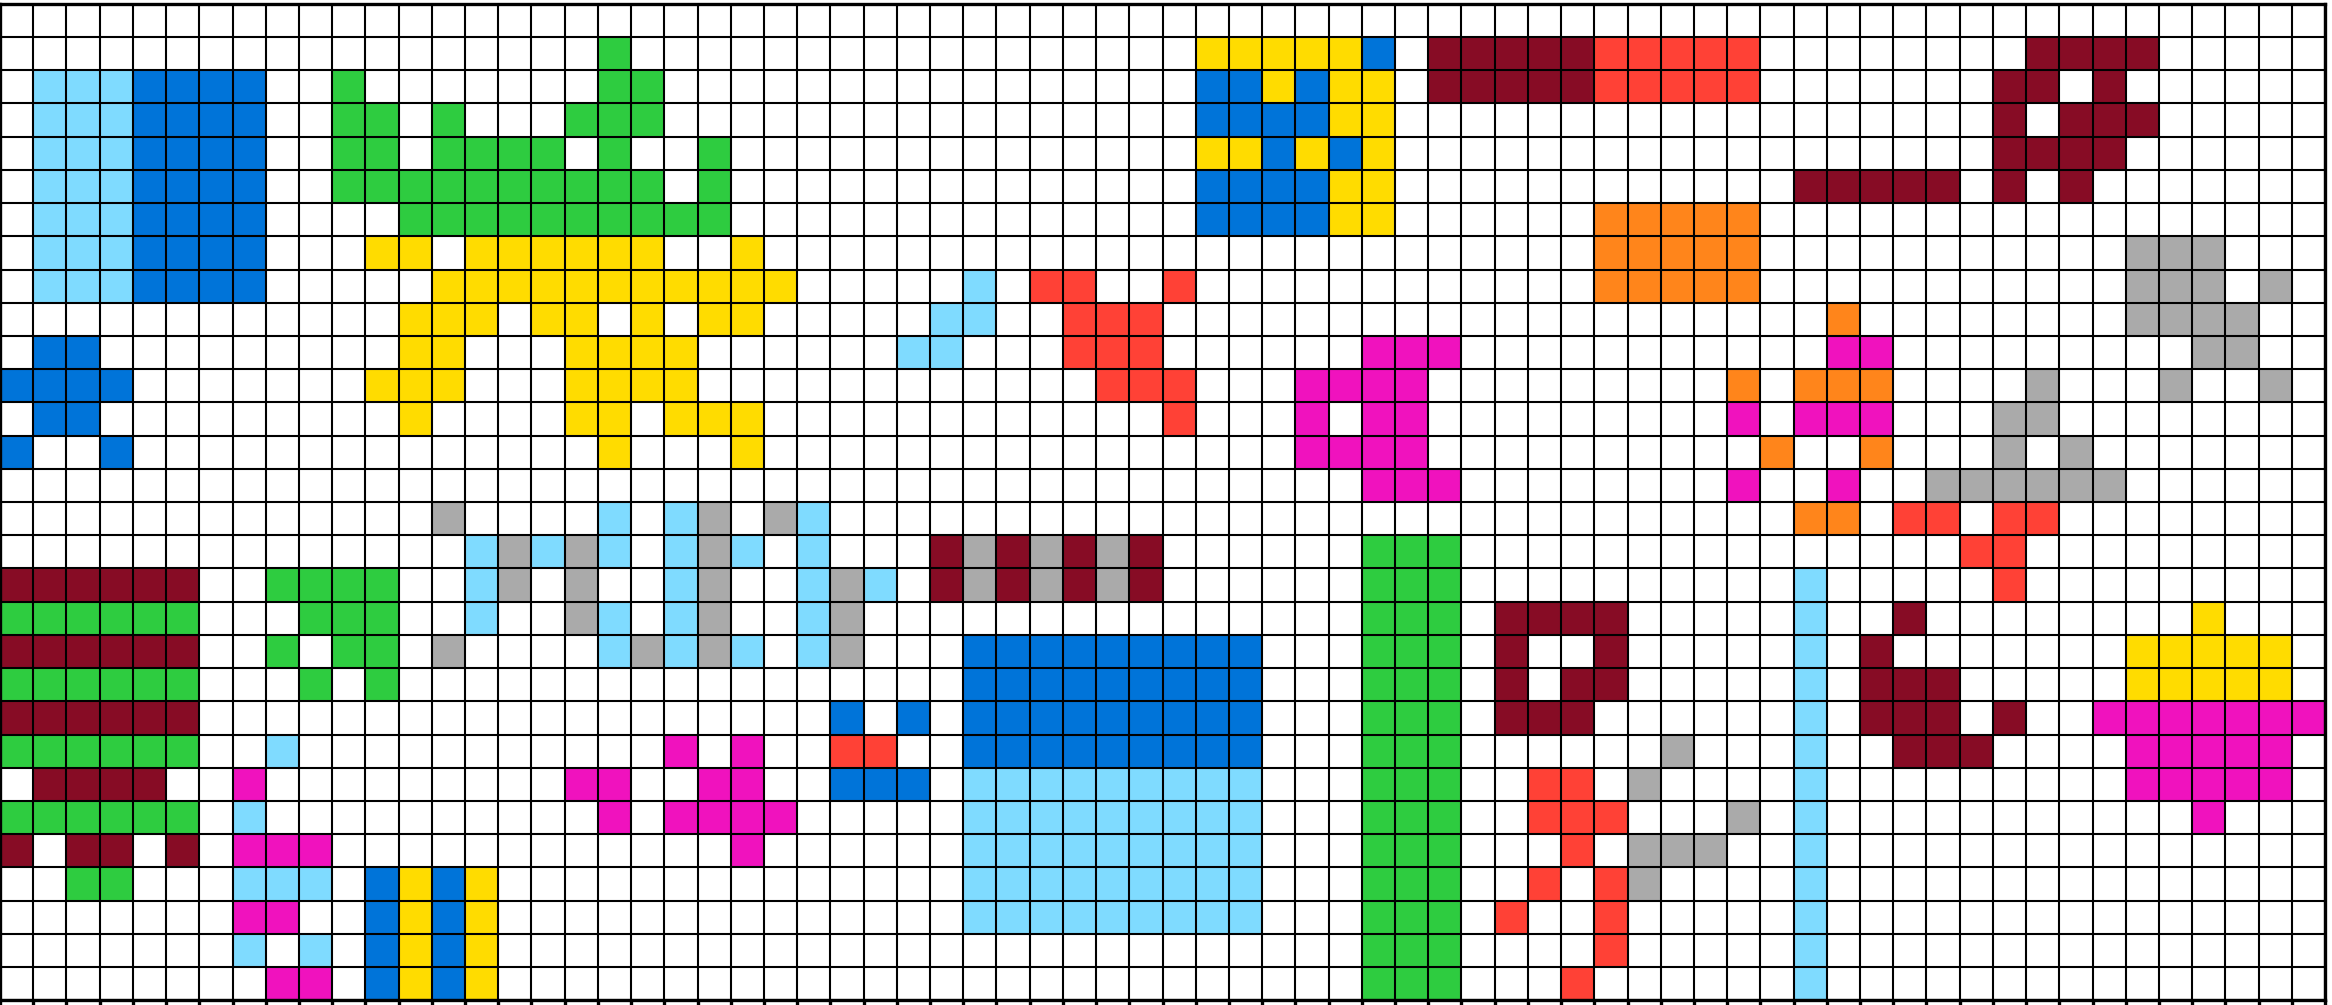
\includegraphics[width=0.9\columnwidth]{Figures/objects.png}
    \caption{Random example of generated objects. The objects are generated with a variety of properties, including size, symmetry, connectivity, colors, color patterns, and footprints. Note: objects are not allowed to overlap, touch, or be inside one another in our generator environment, as reflected in the above image.}
    \label{fig:ARC_shapes}
\end{figure}

Rather than generating objects on the fly, which can be more costly computationally, we favor a method where we pre-generate a large set of 23,000 objects, and compute a table of properties that these objects satisfy. This allows us to efficiently sort through objects at generation time with respect to the constraints specified by the user, as well as the object constraints that the transformation suite may impose. We share the file with these objects along with our code publication, as well as the code used to generate these, so the community can expand the number of objects at will. Below are all the properties through which we iterate, creating combinations of every single parameter, up until a maximum object dimension of 15$\times$15 pixels. 

\begin{itemize}[itemsep=3pt, parsep=0pt, topsep=0pt]
    \item \textbf{Size:} Number of rows, columns, and pixels. 
    \item \textbf{Symmetry}: Horizontal, vertical, diagonal, point, and no symmetry. 
    \item \textbf{Connectivity}: "4 connected" (only connected through adjacent edges), "8 connected" (only connected through adjacent or diagonal edges), or even "distance" (object can be composed of unconnected blocks).
    \item \textbf{Colors}: Single colored or multi-colored.
    \item \textbf{Color Pattern}: Uniform (single color), column stripes, row stripes, diagonal stripes, top-bottom coloring (object split in two colors), right-left coloring (object split in two colors), or random. 
    \item \textbf{Footprints}: Predefined objects such as rectangle, disk, square, diamond, or ellipse. 
\end{itemize}

\subsection{COGITAO Transformations}\label{appendix:COGITAO_transformations}


We provide a set of \ntransforms\ object-transformations, which the community can further expand. As noted in the main manuscript, each transformation was chosen to respect two core rules: (1) each transformation should be composable with all other transformations; and (2) each transformation should modify the object in a way that should not be systematically equivalent to a combination of other transformations. Rule 1 is critical to ensure that our generator maximizes the number of possible tasks that can be generated and avoids degenerate cases. Rule 2 avoids redundancy in the transformations - for instance, we could have implemented an individual transformation \texttt{translate\_up\_right}, but this would always be equivalent to the transformation sequence \texttt{translate\_up} and \texttt{translate\_right}. Rule 2, however, doesn't imply that each transformation suite \textit{necessarily} yields a unique output grid that could not have been reached with another transformation suite. For instance, for symmetric objects, applying mirror transformations could yield the same output objects as applying the rotation transformations twice - this is not the case for non-symmetric objects, thereby still satisfying Rule 2. We refer the reader to Appendix \ref{appendix:transformation_learnability} for an evaluation of the learnibility of each of the transformations. 

We summarize below all 10 families of transformations available in the generator, and a description of the available variations.

\begin{itemize}
    \item \textbf{Translate} (Up, Down, Left, and Right): Translates the entire object by one pixel in any of the 4 dimensions. 
    
    \item \textbf{Mirror} (Horizontal and Vertical): Mirrors the object with respect to the vertical or the horizontal symmetry axis. 
    
    \item \textbf{Rotate} (90 degrees): Rotates the object by 90 degrees.
    
    \item \textbf{Crop} (Top Side, Bottom Side, Right Side, Left Side, Contours): Crops the object's specified side(s). 
    
    \item \textbf{Change Color} ($\texttt{mod } 9 + 1$): Changes object color to $\texttt{new\_color} = \texttt{original\_color} \texttt{mod } 9 + 1$ (e.g., if the object's color is 7, it is changed to the color 8).
    
    \item \textbf{Fill} (Same Color, Different Color): Fills object holes with its color, or the $\texttt{mod } 9 + 1$ color.
    
    \item \textbf{Empty}: Empties inside of the object, and leaves contours. 
    
    \item \textbf{Extend}(Same Color, Different Color): Extends the outermost edges of the object with either the same color or ($\texttt{mod } 9 + 1$) color. 
    
    \item \textbf{Pad} (Top, Bottom, Left, Right, Full object): Pads in the specified direction with a fixed color.
    
    \item \textbf{Duplicate} (Top, Bottom, Left, Right, Quadruple): Duplicates the object in the specified direction. 
\end{itemize}

\paragraph{Note regarding the $\texttt{mod } 9 + 1$:} 

Object colors take values $c \in \{1, \dots, 9\}$, with $c = 0$ reserved for \textbf{background}. The color-change operation $\texttt{mod } 9 + 1$ is defined as a cyclic increment over the nine object colors:

$$
c' =
\begin{cases}
((c - 1) \bmod 9) + 1, & c \in \{1,\dots,9\} \\
0, & c = 0 .
\end{cases}
$$

This rule increments each object color by one in a cyclic fashion (sending $9 \mapsto 1$) while ensuring that the background value remains unchanged. Every transformation that involves a color change (e.g. \texttt{change\_color, fill, extend, pad}) follows this rule - which is fully deterministic and easily learnable by models.


\subsection{COGITAO Generation Algorithm}\label{appendix:COGITAO_generation}

Below is an outline pseudocode of the \generatorName\ generation framework.  

\begin{algorithm}
    \caption{\texttt{GenerateCogitaoTask(init\_params)} - Below is a simplified pseudo-code for the general algorithmic logic of the \texttt{\generatorName} generator: Generator}
    \label{before-arc-algorithm}
    \begin{algorithmic}[1] % The number tells where the line numbering should start
        \For {d in transformation\_depth}
            \State transformation\_suite $\gets \texttt{sampleTransformations}(\text{init\_params, possible\_transformations})$
            \EndFor
        \While {trial\_n < max\_trials \ $\&$ \ example\_n $\leq$ wanted\_examples}
            \State input\_grid, objects $\gets \texttt{setInitialGrid}(\text{init\_params, transform})$
            \State output\_grid $\gets$ input\_grid
            \For {object in objects}
                \For {transformation in transformation\_suite}
                    \State output\_grid $\gets \texttt{transformAndPosition}(\text{output\_grid, object, transformation})$
                \EndFor
            \EndFor
            \State task $\gets \text{(input\_grid, output\_grid, transformation\_suite)}$
        \EndWhile
        \State \textbf{Return:} task, transform 
    \end{algorithmic}
\end{algorithm}

The \texttt{sampleTransformations()} function simply iterates through the pool of transformations at the desired depth $d$ to create the transformation sequence. An important function of our algorithm is \texttt{setInitialGrid()}, which sets up the randomly sampled objects in the grid given the init\_params (e.g. number of objects, desired object properties) and the sampled transformation sequence. Indeed, each transformation is defined with a set of object constraints, which are object properties for which the transformation can be applied without ambiguity. This function thus ensures that the random sampling of objects aligns with the sampled transformation sequence to avoid unexpected errors. The \texttt{setInitialGrid()} function positions objects to keep them fully within the grid and to avoid contact with other objects. Finally, the \texttt{transformAndPosition} function applies the transformations to objects and positions them back to the grid. Importantly, this function verifies that the transformed objects are still fully within grid dimension and do not collide with other objects (although adjacent contact is allowed at the transformation stage). If contact occurs, or objects go out of bounds, the entire input-output pair is discarded and generation is restarted. 

For a standard 20x20 grid, with 4 objects (smaller than 6x6) and a sequence of 2 transformations applied, the average input-output pair generation time is at $0.005s \pm 0.002s$ \footnote{These figures were obtained on an Ubuntu 22.04.5 LTS machine equipped with two AMD EPYC 7742 64-Core Processors (128 cores total) running at up to 2.25 GHz, and 256 GB of system RAM}. Some configurations are more difficult and therefore more time-consuming to generate. For instance, decreasing the grid size and increasing the number of objects can significantly increase the generation time. Some transformation combinations are also more challenging to generate, such as series of object duplications which quickly yield objects too large for the grids. 